\documentclass[12pt, oneside]{article}
\usepackage[letterpaper, margin=1in, headsep=0.5in]{geometry}
\usepackage[english]{babel}
\usepackage[utf8]{inputenc}
\usepackage{amsmath}
\usepackage{amsfonts}
\usepackage{amssymb}
\usepackage{tikz}
\usetikzlibrary{angles}

\usepackage{fancyhdr}
\pagestyle{fancy}
\fancyhf{}
\rhead{\thepage \\}
\lhead{BECA / Dr. Huson / Mathematics\\* Template geometric figures}

\renewcommand{\headrulewidth}{0pt}

\begin{document}
\subsection*{Graphs}
tikz grid command

%Graph / grid
\begin{center}
  
\begin{tikzpicture}[scale=0.4] %[xscale=1,yscale=1]
  \draw[step=0.25in,gray,very thin] (0,0) grid (12.7,12.7);
  \end{tikzpicture}
\end{center} %Regents style, no axes

Axes
\begin{figure} %[!htbp]
  \caption{$x$ and $y$ axes for grid}
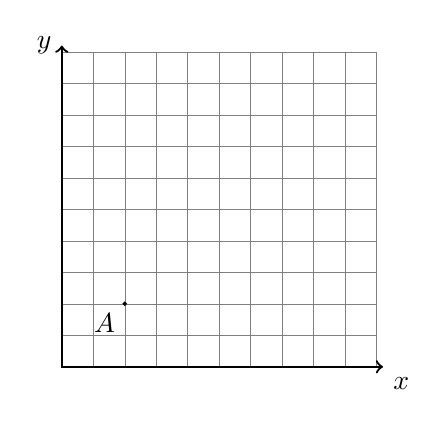
\begin{tikzpicture}[scale=0.4]
  \draw [help lines] (0,0) grid (10,10);
  \draw [thick, <->] (0,10.2) node [left] {$y$}
       -- (0,0) -- (10.2,0) node [below right] {$x$};
  \draw[fill] (2,2) circle  [radius=0.05]
       node[below left] (2, 2) {$A$};
\end{tikzpicture}
\end{figure}

\subsection*{Drawing lines and shapes}
tikz draw command, node labeling function

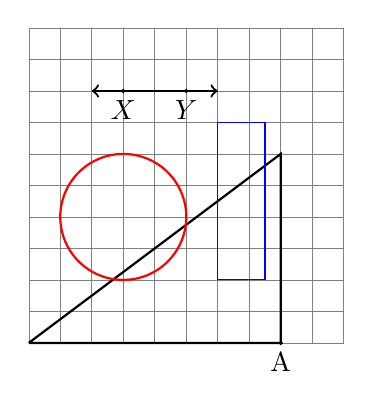
\begin{tikzpicture}[scale=0.4]
  \draw [help lines] (0,0) grid (10,10);
  %Triangle
  \draw [thick](0,0)--(8,0)--(8,6)--(0,0);
  \draw [fill] (8,0) circle [radius=0.05];
  \node [below] at (8,0) {A}; %above, right, left
  %line through points
  \draw [<->, thick] (2,8)--(6,8); % also thin, ultra thick, help lines, dashed, dotted, red
  \draw [fill] (3,8) circle [radius=0.05] node[below]{$X$};
  \draw [fill] (5,8) circle [radius=0.05] node[below]{$Y$};
  %shapes
  \draw [blue] (6,2) rectangle (7.5,7);
  \draw [red, thick] (3,4) circle [radius=2];
\end{tikzpicture}

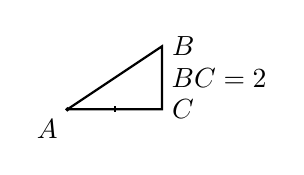
\begin{tikzpicture}[scale=0.4]
  \draw[fill] (2,2) circle  [radius=0.05]
       node[below left] (2, 2) {$A$};
  \draw [thick] (2,2)--(5,2) node[right] {$C$} --(5,4) node[right] {$B$} --(2,2);
  \draw [thick] (3.5,2.1)--(3.5,1.9); %tick mark
  \node [right] at (5,3) {$BC=2$};
\end{tikzpicture}

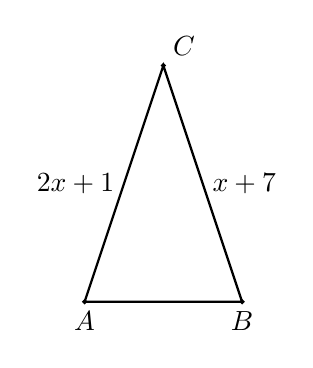
\begin{tikzpicture}[scale=0.5]
  %\draw [help lines] (0,0) grid (10,10);
  %Triangle
  \draw [thick](0,0)--(4,0)--(2,6)--(0,0);
  \draw [fill] (0,0) circle [radius=0.05] node[below]{$A$};
  \draw [fill] (4,0) circle [radius=0.05] node[below]{$B$};
  \draw [fill] (2,6) circle [radius=0.05] node[above right]{$C$};
  \node [right] at (3,3){$x+7$};
  \node [left] at (1,3){$2x+1$};
\end{tikzpicture}

\subsection*{Marking angles}
\tikz \draw (2,0) coordinate (A) -- (0,0) coordinate (B)
         -- (1,1) coordinate (C)
  pic [draw, ->] {angle=A--B--C}; %pic ["$K$"] naming not working


\end{document}
